\documentclass[asi]{picINSA}
\usepackage{pdfpages}

% \input{commandes}

\usepackage{../../../ressources/Unipik/vocabulaire/vocabulaireUnipik}

\definecolor{gris}{gray}{0.75}% utilisé dans les annexes A B et C
\definecolor{gris2}{gray}{0.85}% utilisé dans les annexes A B et C

\titreGeneral{\pgc}
\sousTitreGeneral{\nomEquipe}
\titreAcronyme{\pgcCourt}
\version{V1.00}
\referenceVersion{\pgcCourt\_Q\_\nomEquipe\_\versionPrive}
\titreDetaille{\pgcCourt\_Q\_\nomEquipe\_\versionPrive}
\auteurs{\Mathieu{}}
\destinataires{\nomApprobateur{}, \nomTuteurQualite, \nomEquipe, \nomPIC}
\resume{Le présent document contient la présentation du système de gestion
des configurations pour \nomEquipe.}
\natureDerniereModification{Correction}
\motsCles{\pgcCourt{}, référentiel, nommage}
\modeDiffusionControle{}

\newcommand{\elementRDF}[1]{\NoAutoSpaceBeforeFDP{#1}}

%opening

%Ces deux lignes empèche LaTeX de numéroter les chapitres qui sont inexistant dans le PQ
%makeatletter\@addtoreset{section}{part}\makeatother
%renewcommand{\thesection}{\arabic{section}}

\begin{document}
 \couverture{}
 \informationsGenerales{}
  \begin{pagesService}
  \begin{historique}
    \unHistorique{1.00}{22/01/2016}{\Mathieu}{Création}{Toutes}
  \end{historique}
  
  % \begin{suiviDiffusions}
  % \unSuivi{1.00}{XX/XX/2016}{\nomTuteurQualite{},  \nomApprobateur{}, \nomEquipe{}, \nomPIC{}}
  % \end{suiviDiffusions}
  
  \begin{signatures}
    \uneSignature{Vérificateur}{\RQ{}}{\Pierre{}}{XX/01/2016}{courriel}
    \uneSignature{Validateur}{\CP{}}{\Sergi{}}{XX/01/2016}{courriel}
    \uneSignature{Approbateur}{Direction Qualité de l'Unité P3}{\nomApprobateur{}}{XX/XX/2016}{courriel}
  \end{signatures}
  
  
  \begin{documentsReference}
    \begin{listeDeReferences}
      \uneReference{Norme de management de la qualité}{\isoNeufMilleUn}
      \uneReference{\manuelQualite{} de l'Unité P3}{ASI-MQ-MQASI}
      \uneReference{\dgq{} du Processus Réaliser les PIC}{ASI-DGQ-DGQ2}
      \uneReference{\smq{}}{ISO 10007:2003}
    \end{listeDeReferences}
  \end{documentsReference}
  
  
  \begin{terminologie}
    \begin{listeDAbreviations}
      \uneAbreviation{\ASICourt}{\ASI}
      \uneAbreviation{\CDRCourt}{\CDR}
      \uneAbreviation{CP}{Carnet de Produit ou Chef PIC}
      \uneAbreviation{CR}{Compte-rendu}
      \uneAbreviation{\CRCCourt}{\CRC}
      \uneAbreviation{\CRECourt}{\CRE}
      \uneAbreviation{\CRICourt}{\CRI}
      \uneAbreviation{\CRIPCourt}{\CRIP}
      \uneAbreviation{\CRTPCourt}{\CRTP}
      \uneAbreviation{\CRTQCourt}{\CRTQ}
      \uneAbreviation{CTFT}{Commission de Traitement des Faits Techniques}
      \uneAbreviation{DAC}{Dossier d'Audit de Code}
      \uneAbreviation{DC}{Dossier de conception}
      \uneAbreviation{\DGPCourt}{\DGP}
      \uneAbreviation{\DGQCourt}{\DGQ}
      \uneAbreviation{\DGQUNCourt}{Processus Rechercher, choisir et contractualiser les PIC}
      \uneAbreviation{\DGQDEUXCourt}{Processus Réaliser les PIC}
      \uneAbreviation{\DGQTROISCourt}{Processus Manager la Qualité}
      \uneAbreviation{\DSECourt}{\DSE}
      \uneAbreviation{\DSICourt}{\DSI}
      \uneAbreviation{\DSQCourt}{\DSQ}
      \uneAbreviation{DT}{Dossier de Tests}
      \uneAbreviation{DTI}{Dossier de Tests d'Intégration}
      \uneAbreviation{DTU}{Dossier de Tests Unitaires}
      \uneAbreviation{DTV}{Dossier de Tests de Validation}
      \uneAbreviation{EC}{État de Configuration}
      \uneAbreviation{\FCCourt}{\FC}
      \uneAbreviation{FDO}{Fiche D'Opportunité}
      \uneAbreviation{FDR}{Fiche De Risque}
      \uneAbreviation{\FFCourt}{\FF}
      \uneAbreviation{\FFTCourt}{\FFT}
      \uneAbreviation{FOC}{Fiche d'Ordre de Correction}
      \uneAbreviation{\FRCourt}{\FR}
      \uneAbreviation{GC}{Gestion des Configurations}
      \uneAbreviation{GP}{Gestion de Projet}
      \uneAbreviation{GU}{Guide Utilisateur}
      \uneAbreviation{I}{Implémentation}
      \uneAbreviation{IHM}{Interface Homme Machine}
      \uneAbreviation{\INSACourt}{\INSA}
      \uneAbreviation{ISO}{International Standard Organisation}
      \uneAbreviation{LC}{Livraisons Complémentaires}
      \uneAbreviation{lotX}{Lot numéro X}
      \uneAbreviation{MC}{Mail du client}
      \uneAbreviation{MDQ}{Mail du Directeur Qualité}
      \uneAbreviation{\MGPICourt}{\MGPI}
      \uneAbreviation{ML}{Mail de Livraison}
      \uneAbreviation{MP3}{Mail de l'unité P3}
      \uneAbreviation{\MQCourt}{\MQ{} du departement \ASI}
      \uneAbreviation{MTP}{Mail du Tuteur Pédagogique}
      \uneAbreviation{MTQ}{Mail du Tuteur Qualité}
      \uneAbreviation{\OCCourt}{\OC}
      \uneAbreviation{OF}{Organigramme Fonctionnel}
      \uneAbreviation{\PDFCourt}{\PDF}
      \uneAbreviation{PERT}{Project Evaluation and Review Technique}
      \uneAbreviation{PGC}{Plan de Gestion des Configurations}
      \uneAbreviation{\PICourt}{\PI}
      \uneAbreviation{\PICCourt}{\PIC}
      \uneAbreviation{\PQCourt}{\PQ}
      \uneAbreviation{PRO}{Portefeuille des Risques et Opportunités}
      \uneAbreviation{PTI}{Plan de Tests d'Intégration}
      \uneAbreviation{PTU}{Plan de Tests Unitaires}
      \uneAbreviation{\PTVCourt}{\PTV}
      \uneAbreviation{\PVCourt}{\PV}
      \uneAbreviation{PVD}{Procès-verbal de démarrage}
      \uneAbreviation{PVDSE}{Procès-Verbal de Document de Spécification Externe}
      \uneAbreviation{PVDSI}{Procès-Verbal de Document de Spécification Interne}
      \uneAbreviation{PVFPCP}{Procès-Verbal de Fin de Phase de Conception Préliminaire}
      \uneAbreviation{PVFPI}{Procès-Verbal de Fin de Phase d'Intégration}
      \uneAbreviation{PVFPS}{Procès-Verbal de Dossier de Fin de Phase de Spécification}
      \uneAbreviation{PVPTV}{Procès-Verbal de Plan de Tests de Validation}
       \uneAbreviation{PVR}{Procès-Verbal des Recettes}
      \uneAbreviation{QSC}{Questionnaire de Satisfaction Client}
      \uneAbreviation{RAI}{Rapport d'Audit Interne}
      \uneAbreviation{\RDSECourt}{\RDSE}
      \uneAbreviation{\RDSICourt}{\RDSI}
      \uneAbreviation{\RFDCourt}{\RFD}
      \uneAbreviation{\RFFPCPCourt}{\RFFPCP}
      \uneAbreviation{RFFPI}{Revue Formelle de Fin de Phase d’Intégration}
      \uneAbreviation{\RFFPSCourt}{\RFFPS}
      \uneAbreviation{RFR}{Revue Formelle des Recettes}
      \uneAbreviation{revueX}{Revue numéro X}
      \uneAbreviation{\SMQCourt}{\SMQ}
      \uneAbreviation{SP}{Support Présentation}
      \uneAbreviation{\TBCourt}{\TB}
      \uneAbreviation{Unité P3}{Unité de Pédagogie Par Projets}
      \uneAbreviation{WBS}{Work Breakdown Structure}
    \end{listeDAbreviations}
  \end{terminologie}
\end{pagesService}

 \tableofcontents
 
 \chapter*{Introduction}
 \newcommand{\gcLong}{Gestion des Configurations}

\section*{Objet}
L'objectif de ce document est de présenter les principes et les procédures nécessaires à la mise en œuvre de la gestion des configurations prévue par la norme \isoNeufMilleUn.

\section*{Définition}

Le présent document établit les règles et la structure de la gestion des configurations qui doivent être suivies pendant toute la durée du \picCourt. Il contient :
\begin{itemize}
\item les règles de nommage;
\item la description des différents référentiels;
\item les règles spécifiques de \nomEquipe{};
\item la description de l'administration des configurations;
\item la description de la maîtrise des documents;
\item la description de la maîtrise des enregistrements;
\item les règles d'archivage.
\end{itemize}


 
 \chapter{Règles de nommage}
 \label{chap regle nommage}
 Dans le but d'identifier clairement et de manière unique les éléments de configuration du \picCourt{}, il est nécessaire de spécifier des règles de nommage. Chaque élément inclus dans un référentiel doit respecter la règle de nommage qui lui convient.\\

L'ensemble des fichiers suit le modèle suivant :
\[
  <Type>\_<Referentiel>\_Unipik\_<Suffixe>
\]
On utilisera des abréviations pour chaque élément (Type, Référentiel et Suffixe).\\
Par exemple la première version du Plan de Gestion des Configurations aura pour nom de fichier :
\[
PGC\_Q\_Unipik\_v1.00
\]
Et se trouvera dans le dossier :
\[
Unipik/qualite/GP/PGC/
\]

\section{Nom du \picCourt{}}
Ce champ indique l'appartenance du document au \PICCourt{} peu importe sa provenance
 (\PICCourt{}, client, département \ASI{}, etc). Il a pour valeur \textbf{\nomEquipe}.

\section{Référentiels}

Tous les éléments réalisés au cours du PIC appartiennent à l'un des 5 référentiels suivants : Développement, Livraison, Qualité, Ressources et Spécifications.
\begin{table}[H]
\centering
	\begin{tabularx}{11cm}{|X|c|X|}
	\hline
	\rowcolor[gray]{0.85} Référentiel & Abréviation & Nom du dossier sous \git{} \\
	\hline
	Spécifications & S & specifications\\ 
	\hline
	Qualité & Q & qualite\\
	\hline
	Développement & D & developpement\\
	\hline	
	Livraison & L & livraison\\
	\hline 
	Ressources & R & ressources\\
	\hline
	\end{tabularx}
\caption{Abréviations associées à chaque type}
\label{Référentiel}
\end{table}

\section{Types}

\begin{longtable}{|p{12cm}|c|c|}
    \hline
    \rowcolor[gray]{0.85} Documents et Enregistrements & Type & Suffixe 			\endfirsthead
    \hline	
    \rowcolor[gray]{0.85} Documents et Enregistrements & Type & Suffixe \endhead
    \hline
    \multicolumn{3}{|c|}{\textbf{\bsc{suite ...}}}\endfoot
    \hline
    \endlastfoot
    \hline
    \multicolumn{3}{|c|}{\textbf{\bsc{Référentiel Qualité}}}\\
    \hline
    Dossier de Suivi de la Qualité & DSQ & -\\
    \hline
    	\hspace{1cm} Fiche de Fait Technique & FFT & n\\
    \hline
    \hspace{1cm} Fiche de Compétences & FC & p-v\\
    \hline
    \hspace{1cm} Fiche de Formation & FF & c\\
    \hline
    \hspace{1cm} Fiche de Rôle & FR & r-v\\
    \hline
    \hspace{1cm} Organigramme Fonctionnel & OF & v\\
    \hline
    \hspace{1cm} Plan de Formation & PF & v\\
    \hline
    \hspace{1cm} Questionnaire de Satisfaction Client & QSC & d\\
    \hline
    \hspace{1cm} Rapport d'Audit Interne & RAI & d\\
    \hline
    \hspace{1cm} Tableau de Bord & TB & s\\
    \hline
    \hspace{1cm} Fiche d'Indicateurs & FI & n\\
    \hline
    Gestion de Projet & GP & -\\
    \hline
    \hspace{1cm} Compte-Rendu & CR & -\\
    \hline
    \hspace{2cm} Compte-Rendu de réunion Client & CRC & d\\
    \hline
    \hspace{2cm} Compte-Rendu de réunion Exceptionnelle & CRE & d\\
    \hline
    \hspace{2cm} Compte-Rendu de réunion Interne & CRI & d\\
    \hline
    \hspace{2cm} Compte-Rendu de réunion Inter-PIC & CRIP & d\\
    \hline
    \hspace{2cm} Compte-Rendu de réunion Tuteur Pédagogique & CRTP & d\\
    \hline
    \hspace{2cm} Compte-Rendu de réunion Tuteur Qualité & CRTQ & d\\
    \hline
    \hspace{1cm} E-mails & mails & -\\
    \hline
    \hspace{2cm} Mail du Client & MC & d\\
    \hline
    \hspace{2cm} Mail du Directeur Qualité & MDQ & d\\
    \hline
    \hspace{2cm} Mail de Livraison & ML & d\\
    \hline
    \hspace{2cm} Mail de l'Unité P3 & MP3 & d\\
    \hline
    \hspace{2cm} Mail du Tuteur Pédagogique & MTP & d\\
    \hline
    \hspace{2cm} Mail du tuteur Qualité & MTQ & d\\
    \hline
    \hspace{1cm} Procès-Verbal & PV & PV\\
    \hline
    \hspace{2cm} Revue Formelle de Démarrage & RFD & -\\
    \hline
    \hspace{3cm} Procès-Verval de Démarrage & PVD & d\\
    \hline
    \hspace{2cm} Revue Formelle de Fin de Phase de Conception Préliminaire & RFFPCP & -\\
    \hline
    \hspace{3cm} Procès-Verbal de Fin de Phase de Conception Préliminaire & PVFPCP & d\\
    \hline
    \hspace{2cm} Revue Formelle de Fin de Phase d'Intégration & RFFPI & -\\
    \hline
    \hspace{3cm} Procès-Verbal de Fin de Phase d'Intégration & PVFPI & d\\
    \hline
    \hspace{2cm} Revue Formelle de Fin de Phase de Spécification & RFFPS & -\\
    \hline
    \hspace{3cm} Procès-Verbal de Dossier de Spécifications Externes & PVDSE & d\\
    \hline
    \hspace{3cm} Procès-Verbal de Dossier de Spécifications Internes & PVDSI & d\\
    \hline
    \hspace{3cm} Procès-Verbal de Fin de Phase de Spécifications & PVFPS & d\\
    \hline
    \hspace{3cm} Procès-Verbal de Plan de Tests de Validation & PVPTV & d\\
    \hline
    \hspace{2cm} Revue Formelle de Recettes & RFR & -\\
    \hline
    \hspace{3cm} Procès-Verbal de Recettes & PVR & d\\
    \hline
    Gestion des Configurations & GC & -\\
    \hline
    \hspace{1cm} Etat de Configuration & EC & d-c\\
    \hline
    \hspace{1cm} Fiche de Remise de Documents & FRD & d-c\\
    \hline
    \hspace{1cm} Fiche de Remise de Matériels & FRM & d-c\\
    \hline
    \hspace{1cm} Fiche Récapitulative de Référentiel & FRR & s\\
    \hline
    \hspace{1cm} Plan de Gestion des Configurations & PGC & v\\
    \hline
    Portefeuille des Risques et Opportunités & PRO & -\\
    \hline
    \hspace{1cm} Fiche De Risque & FDR & n\\
    \hline
    \hspace{1cm} Fiche D'Opportunité & FDO & n\\
    \hline
    Plan Qualité & PQ & v\\
    \hline
 \multicolumn{3}{|c|}{\textbf{\bsc{Référentiel Spécification}}}\\
    \hline
    LotX & lotX & -\\
    \hline
    \hspace{1cm} Cahier De Recettes & CDR & n-v\\
    \hline
    \hspace{1cm} Carnet de Produit & CP & n-v\\
    \hline
    \hspace{1cm} Dossier de Spécifications Externes & DSE & n-v\\
    \hline
    \hspace{1cm} Cahier De Spécifications Internes & DSI & n-v\\
    \hline
    \hspace{1cm} Plan de Tests de Validation & PTV & n-v\\
    \hline
 \multicolumn{3}{|c|}{\textbf{\bsc{Référentiel Développement}}}\\
    \hline
    Dossier d'Audit de Code & DAC & d\\
    \hline
    Implémentation & I & -\\
    \hline
    LotX & lotX & -\\
    \hline
    \hspace{1cm} Dossier de Conception & DC & v\\
    \hline
    \hspace{1cm} Dossier de Tests & DT & -\\
    \hline
    \hspace{2cm} Dossier de Tests d'Intégration & DTI & n-v \\
    \hline
    \hspace{2cm} Dossier de Tests Unitaires & DTU & n-v \\
    \hline
    \hspace{2cm} Plan de Tests d'Intégration & PTI & n-v \\
    \hline
    \hspace{2cm} Plan de Tests d'Intégration & PTU & n-v \\
    \hline
    \hspace{1cm} Guide Utilisateur & GU & v\\
    \hline
    \hspace{1cm} Procédure d'Installation & PI & v\\
    \hline
 \multicolumn{3}{|c|}{\textbf{\bsc{Référentiel Livraison}}}\\
    \hline
    Livraisons Complémentaires & LC & d\\
    \hline
    Lots & lots & -\\
    \hline
    \hspace{1cm} Lot numéro X & lotX & d\\
    \hline
    Revue & revues & -\\
    \hline
    \hspace{1cm} Revue numéro X & revuesX & -\\
    \hline
    \hspace{2cm} Support Présentation & SP & n\\
    \hline
  \caption{Formalisme des différents Types}
  \label{Formalisme Types}  
\end{longtable}

\section{Suffixes}

Lors du nommage nous utilisons des suffixes adaptés en fonction du type de document. Un document peut avoir plusieurs suffixes, dans ce cas ils sont séparés par un "-". Les suffixes possibles sont les suivants : 

	\begin{table}[H]
		\centering
		\begin{tabularx}{10cm}{|X|c|c|}
		\hline
		\rowcolor[gray]{0.85} Suffixe & Abréviation & Format\\
		\hline
		date & d & dAA-MM-JJ\\
		\hline
		version & v & vX.YY\\
		\hline
		numéro & n & nXXX\\
		\hline
		semaine & s & sXX\\
		\hline
		rôle & r & rRole\\
		\hline
		personne & p & pNom\\
		\hline
		commentaire & c & cCommentaire\\
		\hline
		\end{tabularx}
	\caption{Abréviations associées à chaque suffixe}
	\label{Suffixes}
	\end{table}
	


\subsection{Suffixe Date}
\label{suffixe_date}

Le suffixe de date suit le format \textbf{AA-MM-JJ}. AA pour l'année, MM pour le mois et JJ pour le jour. Ce format permet de classer les documents par ordre chronologique.\\

Exemple : $d16-01-27$ 

\subsection{Suffixe Version}
\label{suffixe_version}

Le suffixe version suit le format \textbf{vX.YY}. X correspond au numéro de version, YY au numéro de révision. Le numéro de version représente le numéro de semestre, en considérant que 1 correspond au semestre 4.2 et 2 au semestre 5.1. Le numéro de révision démarre à 00 et est modifié de la façon suivante : le chiffre des dizaines est incrémenté à chaque modification majeure et le chiffre des unités est incrémenté à chaque révision. Quand le numéro de version est incrémenté, celui des révision repasse à 00.\\

Exemple : $v1.00$

\subsection{Suffixe Numéro}
\label{suffixe_numero}

Le suffixe numéro suit le format \textbf{nXXX}. XXX est un nombre entier compris entre 001 et 999. Il commence à la valeur 001 et est incrémenté à chaque nouveau document.\\

Exemple : $n042$

\subsection{Suffixe Semaine}
\label{suffixe_semaine}

Le suffixe semaine suit le format \textbf{sXX}. XX correspond au numéro de la semaine en cours, la première semaine du PIC étant 01. Seules les semaines comportant au moins un jour ouvré sont numérotées.\\

Exemple : $s09$

\subsection{Suffixe Rôle}
\label{suffixe_role}

Le suffixe rôle suit le format \textbf{rRole} où Role correspond au rôle concerné par le document. Les valeurs possibles pour Role sont : 
\begin{itemize}
\item CP : Chef Projet;
\item CPA : Chef Projet Adjoint;
\item RGC : Responsable Gestion des Configurations;
\item RQ : Responsable Qualité;
\item RQA : Responsable Qualité Adjoint;
\item RR : Responsable Réseau;
\item RD : Responsable Développement;
\item D : Développement;
\item PR : Pilote de Risque.\\
\end{itemize}

Exemple : $rCP$

\subsection{Suffixe Personne}
\label{suffixe_personne}

Le suffixe personne suit le format \textbf{pNom} où Nom correspond au nom de famille de la personne concernée par le document. Dans le cas où plusieurs personnes sont concernées le suffixe aura le format \textbf{pNom1Nom2}.\\

Exemple : $pBaron$

\subsection{Suffixe Commentaire}
\label{suffixe_commentaire}

Le suffixe commentaire suit le format \textbf{cX} où X est le commentaire correspondant au fichier. Par exemple le sujet de la formation pour une Fiche de Formation.\\

Exemple : $cLaTeX$



 \chapter{Structure des référentiels}
 \label{chap struc ref}
  Les référentiels sont stockés selon la structure suivante : 

\begin{figure}[ht]
         \begin{center}
         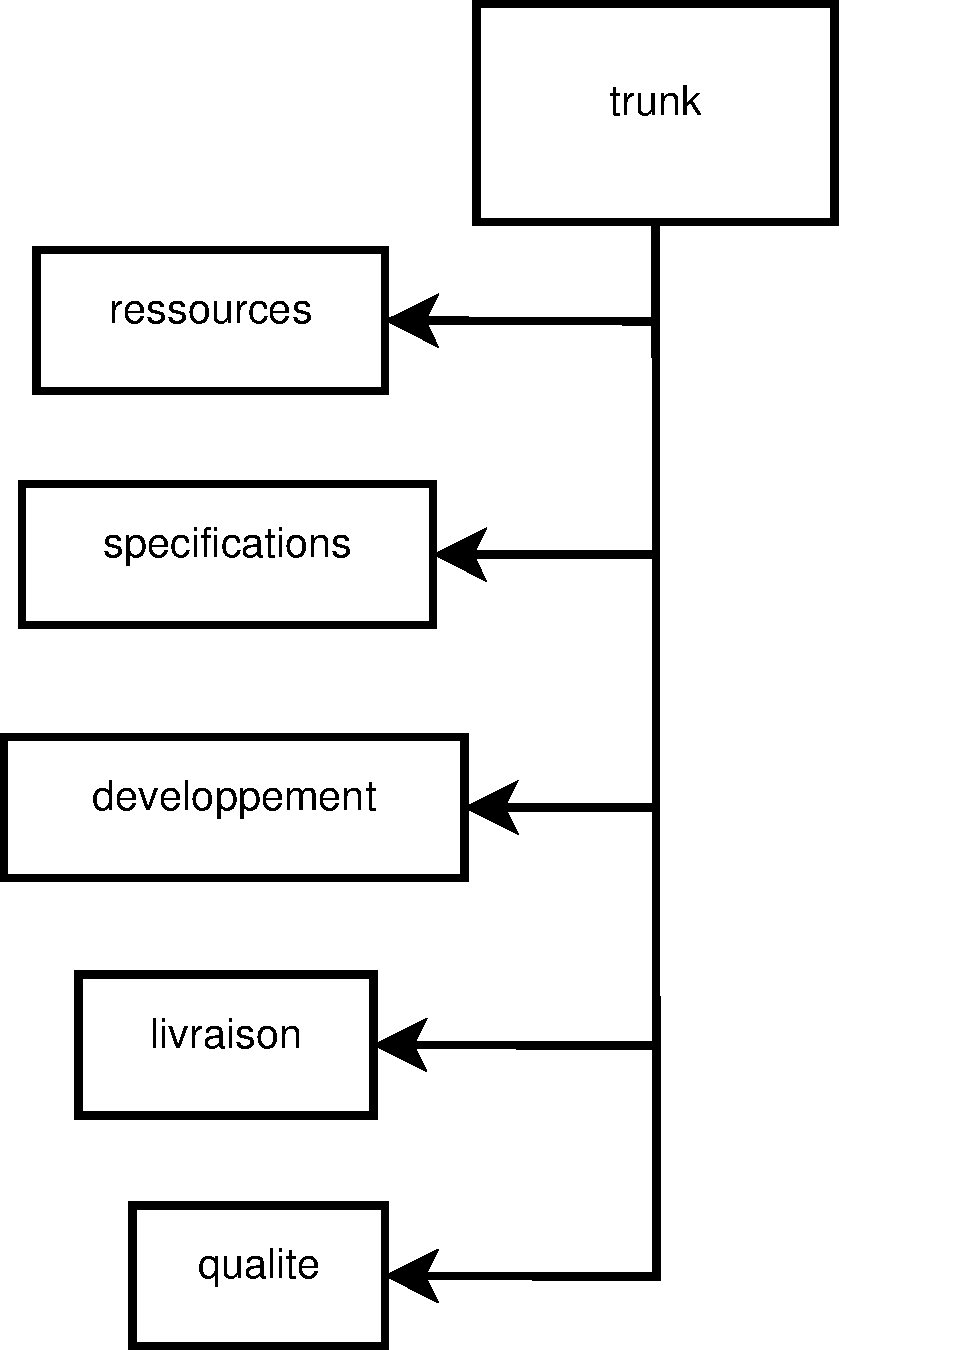
\includegraphics[scale=0.5]{images/arboTrunk}
         \end{center}
         \caption{Structure générale}
 \end{figure}
 
 \section{Référentiel de qualité}
 \subsection{Description}

Le référentiel Qualité contient l'ensemble des documents produit par l'équipe \nomEquipe{}
dans la cadre de sa démarche qualité.

\subsection{Structure générale du référentiel}\label{ref_qualite}



\begin{figure}[ht]
         \begin{center}
         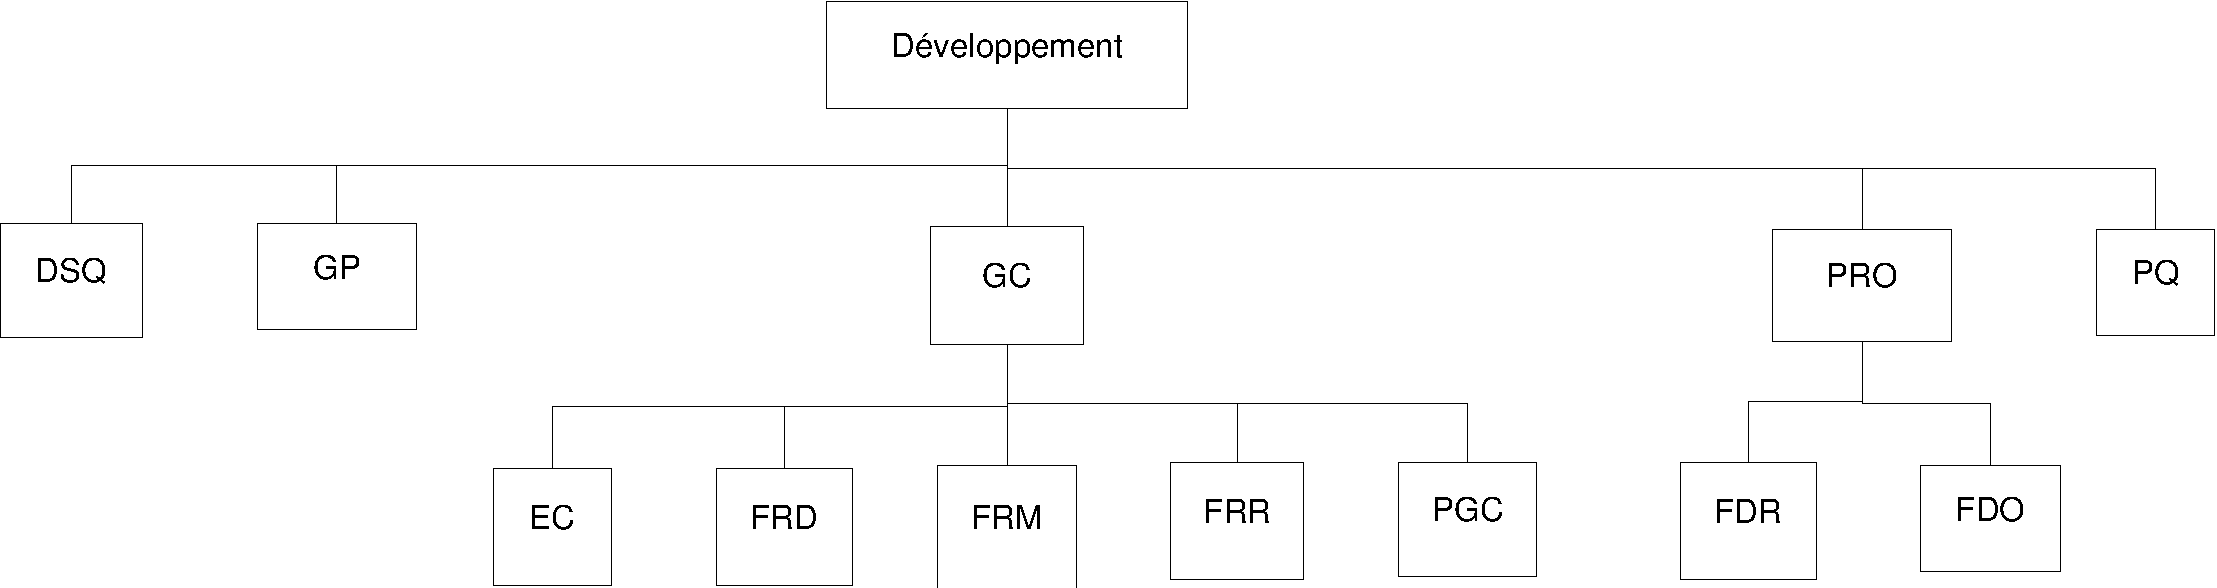
\includegraphics[scale=0.61]{images/arboQualite}
         \end{center}
         \caption{Référentiel Qualité}
 \end{figure}
 
\clearpage

\subsection{Structure du répertoire GP}
\addcontentsline{toc}{subsection}{Structure du répertoire GP}

\begin{figure}[ht]
         \begin{center}
         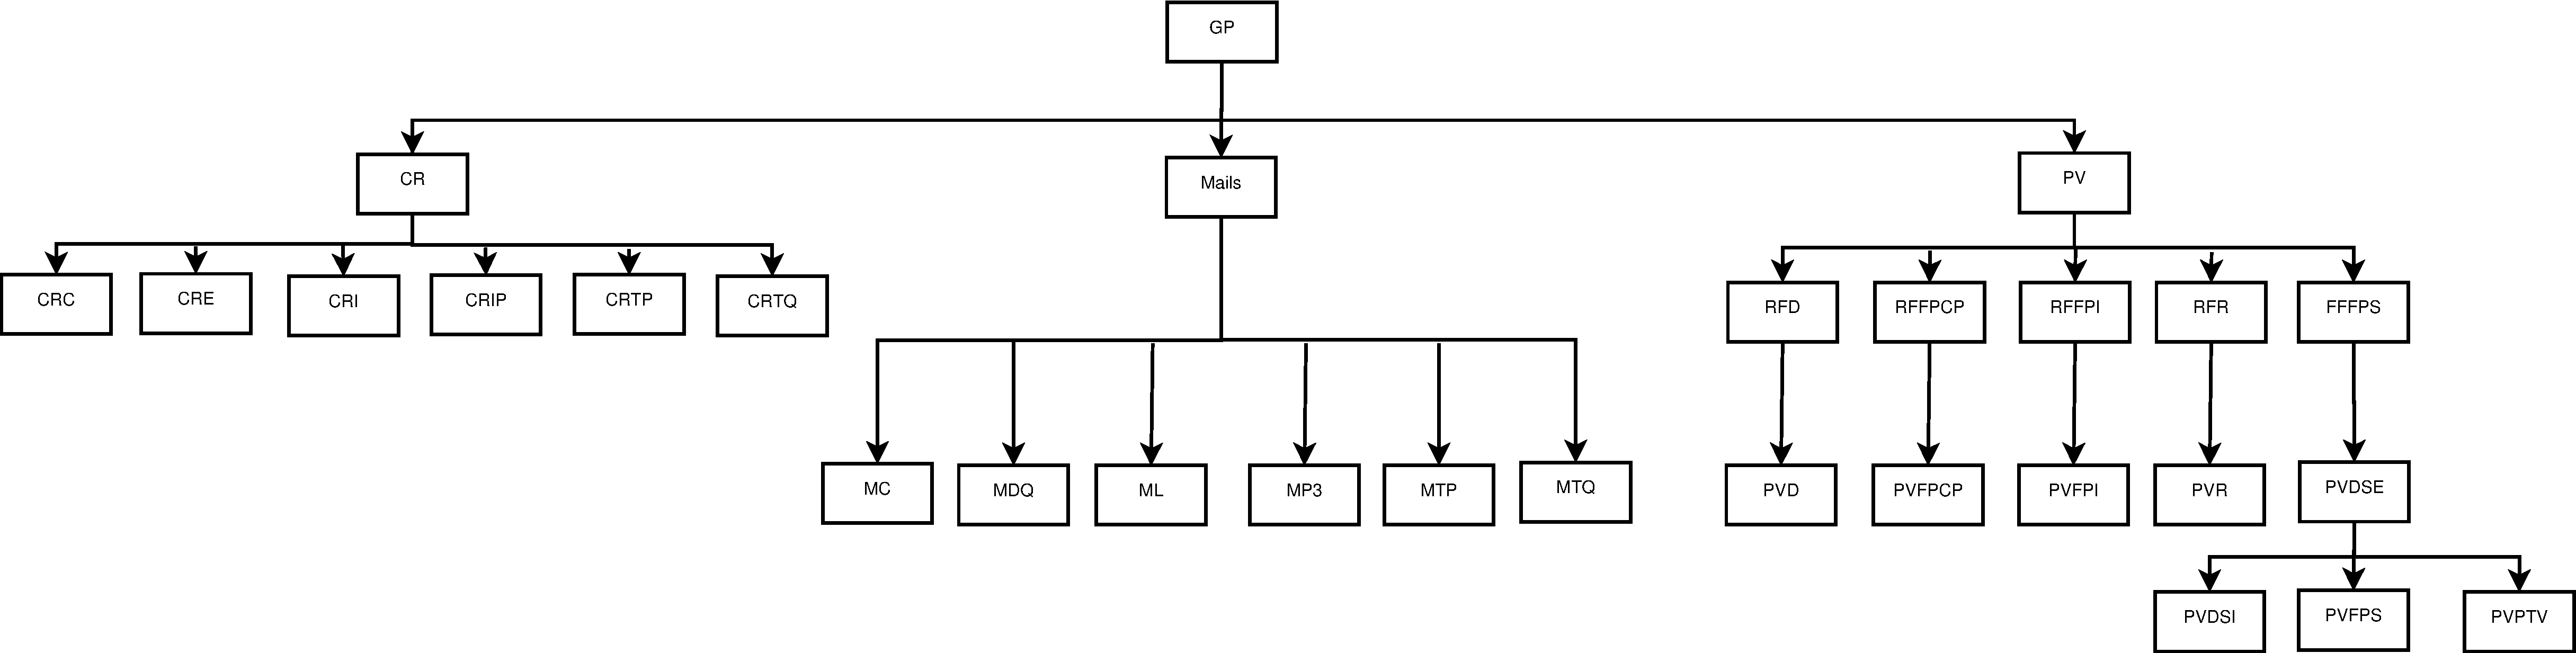
\includegraphics[scale=0.61]{images/arboGP}
         \end{center}
         \caption{Référentiel Qualité - Gestion de Projet}
 \end{figure}
 
 \subsection{Structure du répertoire DSQ}
\addcontentsline{toc}{subsection}{Structure du répertoire DSQ}

\begin{figure}[ht]
         \begin{center}
         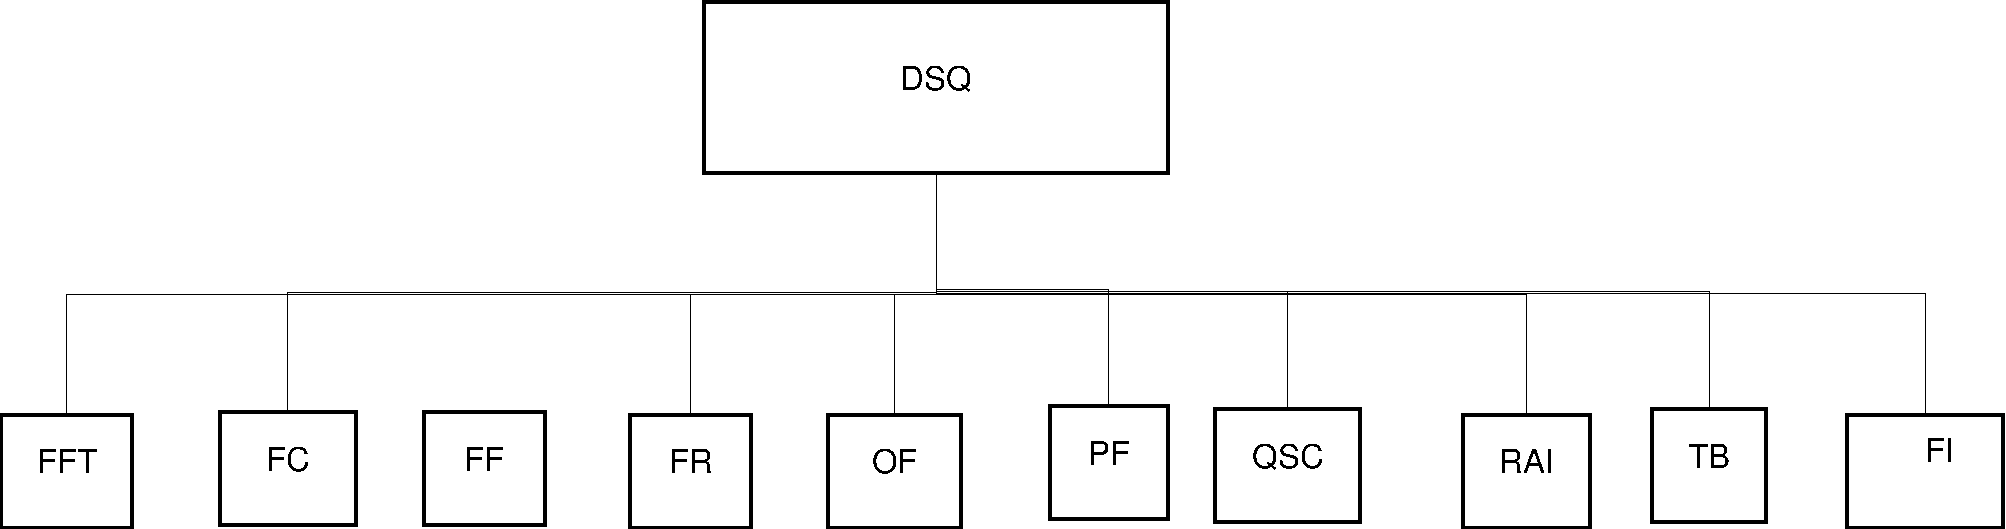
\includegraphics[scale=0.61]{images/arboDSQ}
         \end{center}
         \caption{Référentiel Qualité - Dossier de Suivi de la Qualité}
 \end{figure}


  
 \section{Référentiel de spécifications}
 \section{Description}

Le référentiel Spécification contient l’ensemble des documents réalisés pendant la phase de spécification du \PICCourt. Son arborescence est la suivante:

\section{Structure du référentiel}

\begin{figure}[ht]

         \begin{center}

         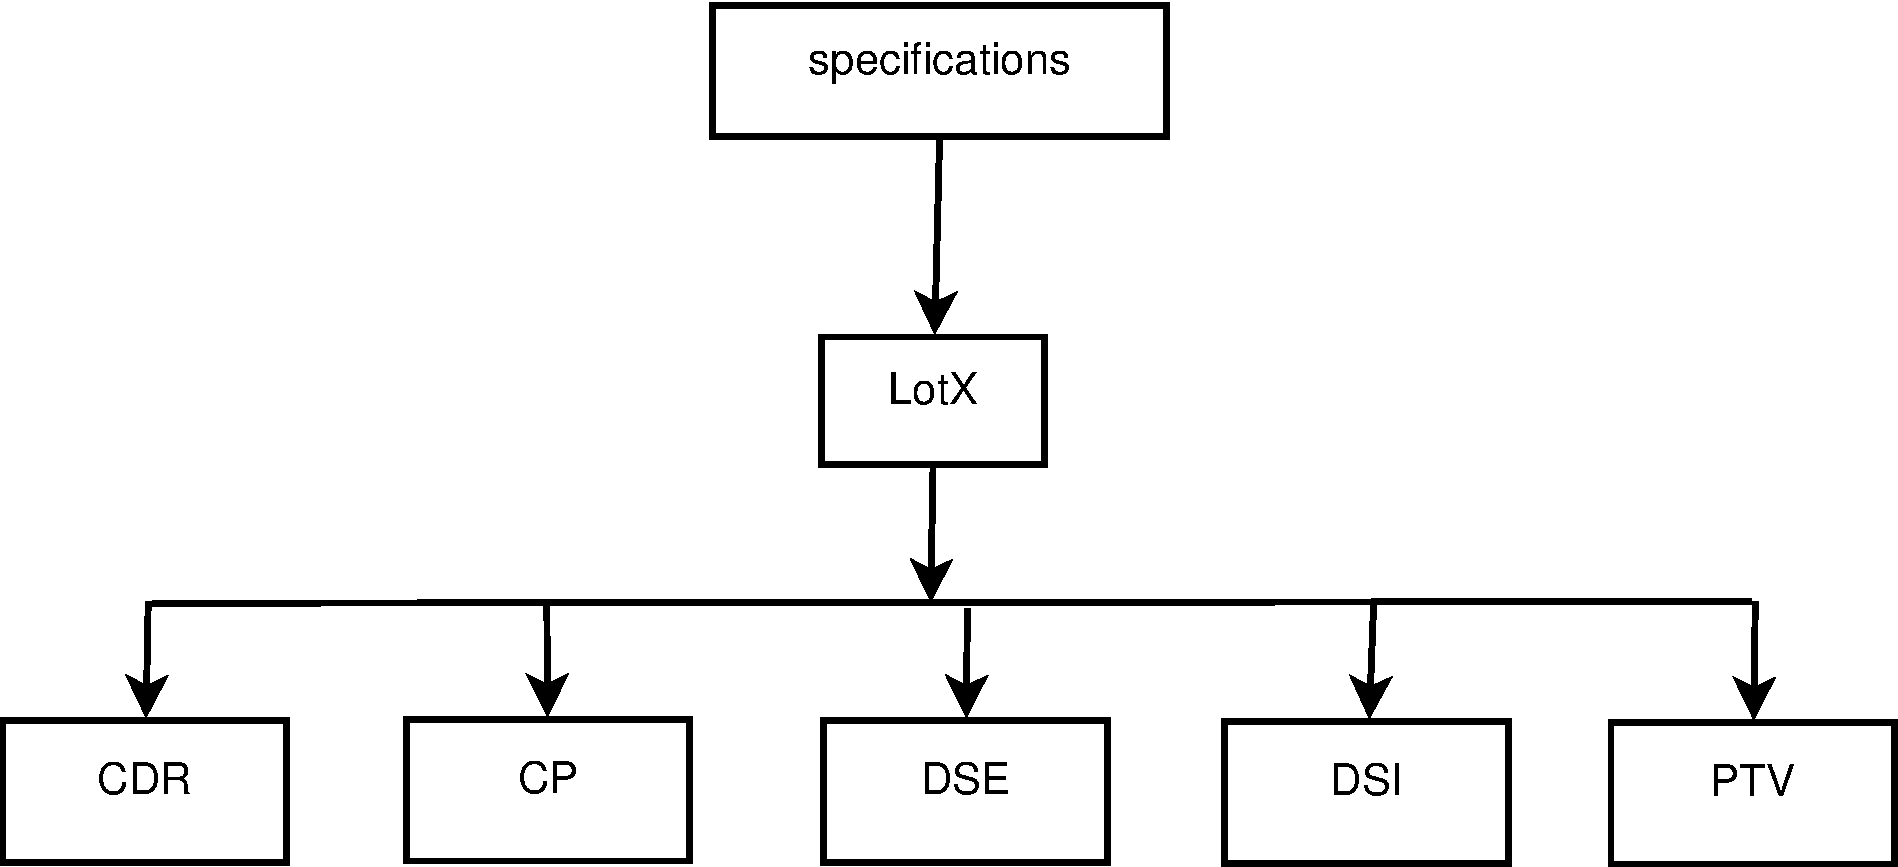
\includegraphics[scale=0.52]{images/arboSpecifications}

         \end{center}

         \caption{Référentiel Spécifications}
 \end{figure}

 
  \section{Référentiel de développement}
 Le référentiel Développement contient l’ensemble des documents réalisés et implémentés au cours du \picCourt.

\clearpage

\begin{figure}[ht]
         \begin{center}
         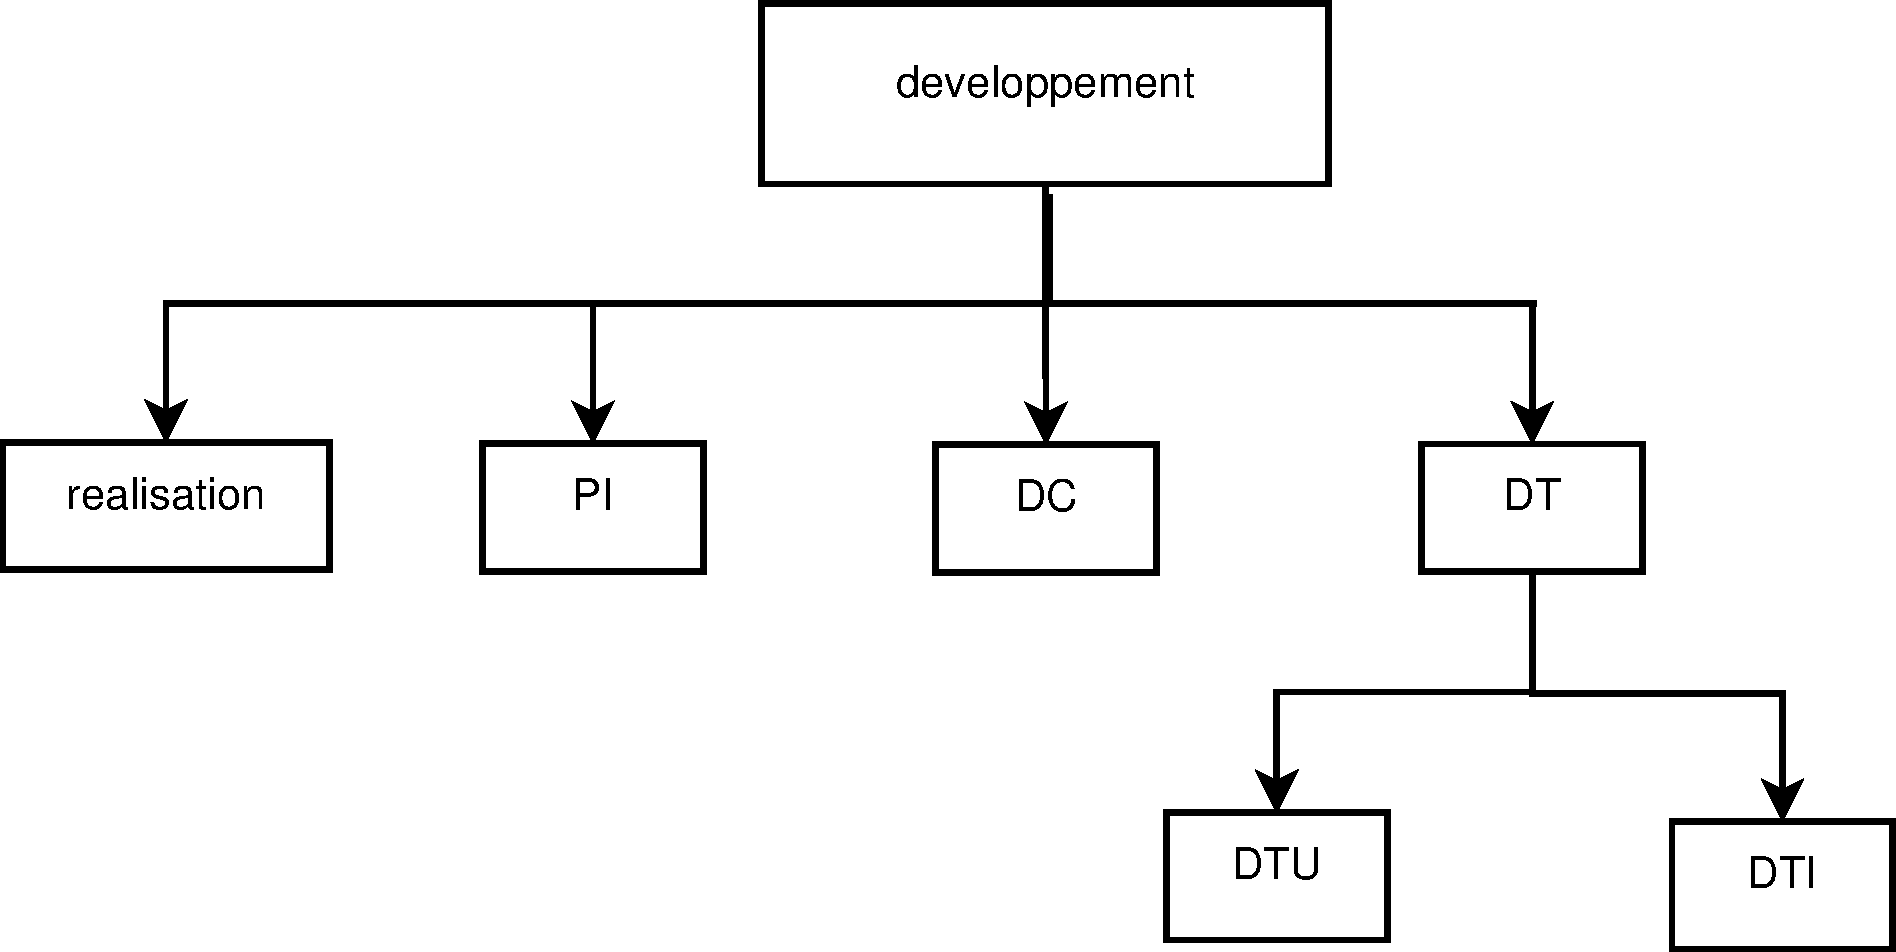
\includegraphics[scale=0.5]{images/arboDeveloppement}
         \end{center}
         \caption{Référentiel Développement}
 \end{figure}

 
  \section{Référentiel de livraison}
 \section{Description}

Le référentiel Livraison contient l'ensemble des livrables de \nomEquipe{}.

\section{Structure du référentiel}\label{ref_livraison}

\begin{figure}[ht]
         \begin{center}
         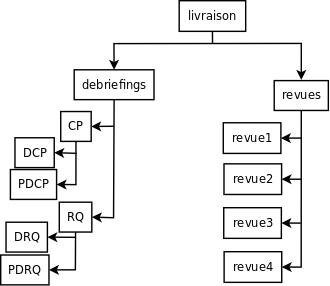
\includegraphics[scale=0.6]{images/I_arboLivraison}
         \end{center}
         \caption{Référentiel Livraison}
 \end{figure}

%\section{Précisions}


%Le répertoire \textbf{livraisons complémentaires} contient les documents livrés au Client
%en dehors des livraisons officielles des lots. Il se trouve dans le \textbf{FTP}.
%Par exemple, si le Client veut prendre connaissance de notre \planQualite{}, 
%il sera placé dans ce répertoire. 
%Ainsi, ce répertoire permettra le traçage de tout ce qui a été envoyé au client en dehors des livraisons.


%~ Le répertoire \textbf{SP}, placé dans le répertoire \textbf{lots}
%~ correspond au support de présentation dans le cas où il y a une présentation orale
%~ de la part de \nomPIC{} pour le Client.

%Pour le cas où une présentation orale est demandée par le Client, 
%le support de présentation sera placé dans le répertoire \textbf{SP}.

 
  \section{Référentiel de ressources}
 \subsection{Description}

Le référentiel Ressources contient l'ensemble des fichiers et des documents utiles au fonctionnement
interne de \nomEquipe{}.

\subsection{Structure du référentiel}

\begin{figure}[ht]
         \begin{center}
         \includegraphics[scale=0.62]{images/I_arboRessources}
         \end{center}
         \caption{Référentiel Ressources}
 \end{figure}

%\section{Précisions}

%Le répertoire \textbf{client} contient l'ensemble des documents fournis par le \client{} à \nomEquipe{}.



 \chapter{Règles spécifiques}
 \label{chap regles specifiques}
  \section{Exception aux règles de nommage}

Le référentiel \textbf{Ressources} ne sera pas soumis aux règles de nommage de \nomEquipe{}, mais une certaines règles doivent être respectées. Chaque dossier et chaque fichier devra être nommé en CamelCase et de manière évoquateur quant au contenu. 

\section{Dossiers spécifiques}

\subsection{Dossiers images}

\`{A} la racine du répertoire des documents nécessitant l'inclusion d'images, de diagrammes ou
d'autres figures, se trouve un répertoire \textbf{images}. Il est ajouté au \git{} par le
rédacteur du document si besoin est. Dans ce répertoire sont stockés les fichiers du projet
(\verb+.dia+, \verb+.xcf+, \verb+.jpg+, etc\dots). Les \verb+.pdf+ de ces fichiers sont générés
à la compilation par le \verb+makefile+.
Les fichiers du répertoire \verb+images+ ne sont pas concernés par les règles de nommage.

\subsection{Dossiers sources}

\`{A} la racine du répertoire des documents nécessitant l'inclusion de sous-fichiers \verb+.tex+
(correspondant à des chapitres, des sections, etc\dots) se trouve un répertoire \textbf{sources} pour
les documents longs nécessitant d'être subdivisés. 
Ces sous-fichiers \verb+.tex+ seront placés dans ce répertoire et ils seront inclus via
le \verb+.tex+ général. Ces sous-fichiers ne sont pas concernés par les règles de nommage.

\subsection{Dossiers annexes}

\`{A} la racine du répertoire des documents nécessitant l'inclusion d'annexes se trouve un répertoire \textbf{annexes}.
Ces documents seront placés dans ce répertoire et ils seront inclus via
le \verb+.tex+ général. Ces sous-fichiers ne sont pas concernés par les règles de nommage.

\subsection{Dossiers pdf}

\`{A} la racine du répertoire de chaque document se trouve un répertoire \textbf{pdf}. C'est
le répertoire dans lequel est placé le \verb+pdf+ généré par la compilation \LaTeX{}. Le \verb+pdf+ n'est pas stocké sur \git{}.

\subsection{Dossiers approbations}

Lorsqu'un document est approuvé par une signature manuscrite, la copie papier de l'enregistrement est archivée dans la salle PIC de  \nomEquipe{} et une numérisation de la page de signatures est effectuée et stockée dans le dossier \verb+approbations+. Les numérisations seront nommées de la manière suivante:
\begin{center}
\verb+ApprobSignature_<Nom du document>+
\end{center}

Exemple : \verb+ApprobSignature_PGC_Q_Unipik_v1.00+

\section{Précisions sur les répertoires de l'arborescence}

\subsection{Répertoire I}

Localisation : \verb+pic_unicef/developpement/I+\\

Le répertoire I (Implementation) est constitué de dossiers représentatifs des différentes applications à produire par le PIC. Le nom de ces dossiers et leur organisation est géré par le responsable développement. Chaque nom de dossier et de fichier doit respecter le nommage camelCase.

\subsection{Répertoire lotX}

Localisations : \\
\verb+pic_unicef/developpement/lotX+\\
\verb+pic_unicef/livraison/lots/lotX+\\

Les répertoires lotX contiendront, en plus des livraisons officielles prévues, le Cahier De Recette du lot concerné annoté par le client.

\subsection{Répertoire client}

Localisation : \verb+pic_unicef/ressources/client+\\

Le répertoire client contient l’ensemble des documents fournis par le client à \nomEquipe.

\section{Règles de rédaction des dates}

Les dates figurant dans les documents sont toutes au format \textbf{JJ/MM/AAAA}. Attention à ne pas confondre avec le format de date des  suffixes dans la convention de nommage (\verb+dAA-MM-JJ+).



 \chapter{Administration des configurations}
  \section{Suivi des configurations}

Afin de permettre le suivi de ces documents ainsi que leur état en temps réel, \nomEquipe{} utilise l'intranet \lintranet. 
Il permet de savoir quelle est la dernière version applicable d'un document et récapitule l'ensemble du contenu des référentiels. 
Cette page est actualisée par la personne concernée lors de la création, la vérification, la validation, l'approbation, la diffusion et l'archivage d'un 
document. 
Sur cette page figurent les informations suivantes:
\begin{itemize}
	\item \textbf{référentiel}: nom du référentiel auquel le document appartient;
	\item \textbf{document}: nom du document;
	\item \textbf{rédacteur}: nom du rédacteur qui a initié le document;
	\item \textbf{vérificateur}: nom du vérificateur;
	\item \textbf{validateur}: nom du validateur;
	\item \textbf{approbation}: le document a été approuvé ou non (case verte si le document a été
	approuvé, rouge sinon);
	\item \textbf{diffusion}: le document a été diffusé ou non (case verte si le document a été
	diffusé, rouge sinon);
	\item \textbf{archivage}: le document a été archivé ou non (case verte si le document a été
	archivé, rouge sinon);
	\item \textbf{référence}: nom complet du document;
	\item \textbf{localisation}: où a été diffusé le document;
	\item \textbf{chemin}: chemin complet d'accès au document sur le \git.
\end{itemize}


\section{L'État de Configuration}

Un État de configuration décrit l'état des documents demandés par leur destinateur à une date donnée. Un état de configuration doit être généré entre autres à chaque livraison. Ils suivent le modèle présenté en \ref{modèle EC}. Chaque fiche comprend un tableau indiquant les informations suivantes pour chaque document :
\begin{itemize}
	\item \textbf{Type}: le type du document. \\
	Exemple : $PQ$ ;
	\item \textbf{Destinataire}: le destinataire du document;
	\item \textbf{Référence du document}: la référence complète du document. \\
	Exemple : $PGC\_Q\_Unipik\_v1.00$;
	\item \textbf{Date de création}: date de création du document.\\
	Format : $JJ/MM/AAAA$ ;
	\item \textbf{Raisons}: le but de l'envoi de ce document.\\
	Exemple : $Livraison\ lot\ 1$.
\end{itemize}


\bigskip
Par sa signature, le vérificateur de l'État de Configuration atteste avoir vérifié la présence
de tous les éléments nécessaires à la livraison ainsi que leur cohérence, tant au niveau de
la forme que du fond.

\paragraph{Précision du suffixe :}
Le suffixe de l'état de configuration est de type commentaire. Ce commentaire doit définir le nom du destinataire. Ceci permettra de retrouver plus facilement les documents envoyés à une personne en particulier.



 \chapter{Maîtrise des documents}
  \section{Historique des évolutions}

Les modifications apportées à un document apparaissent dans sa page de service. À chaque modification il faut indiquer les informations suivantes :
\begin{itemize}
 \item \textbf{version}: indique le numéro de version du document suite à la modification apportée;
\item \textbf{date} : indique la date de la dernière modification du document dans le format \verb+JJ/MM/AAAA+;
\item \textbf{auteur} : indique les noms complets des personnes ayant effectué les modifications;
\item \textbf{modification} : décrit brièvement le type de modification apportée. Si le document a
été diffusé, cette section comprend obligatoirement :
	\subitem \textbullet{ }le numéro de la Fiche d'\OC{} (FOC) qui a donné lieu à la modification;
	\subitem \textbullet{ }le numéro de la Fiche de Fait Technique (\FFTCourt{}) qui lui est associée.
\item \textbf{parties modifiées} : indique les numéros de chapitres et de sections modifiés.
\end{itemize}

\section{Suivi des diffusions}

Le suivi des diffusions est indiqué dans la page de service du document. Il comprend trois informations pour chaque diffusion :
\begin{itemize}
\item \textbf{version} : indique la version du document concerné par la diffusion ;
\item  \textbf{date} : indique la date de diffusion de document ;
\item \textbf{destinataire} : indique les destinataires du document. 
\end{itemize}
 Le suivi des diffusions n’est rempli qu’une fois le document approuvé.

\section{Signatures}

Le contrôle de la vérification, de la validation et de l’approbation d’un document est visible dans la page de service. Il comporte trois lignes correspondant aux trois personnes en charge de ces étapes. Les trois personnes doivent être différentes. L'auteur du document ne peut pas en faire partie.\\

Le \textbf{vérificateur} est responsable de la relecture du document afin d’en vérifier l’orthographe et la cohérence du contenu. Il ne peut en aucun cas être l'auteur du document vérifié..\\

Le \textbf{validateur} évalue la pertinence du document après qu’il ait été vérifié, il engage aussi sa responsabilité en ce qui concerne la correction du document. Il est en charge de la diffusion du document vers les destinaires identifiés et de la mise à jour des dossiers \verb+approbations+.\\

L’\textbf{approbateur} est une personne externe au \pic{}, en charge de l’acceptation du document.

Pour chacune des trois étapes doivent apparaître les informations suivantes dans la page de service :
\begin{itemize}
\item \textbf{fonction} : la fonction de la personne ayant effectué l’étape ;
\item  \textbf{nom} : le nom de la personne ayant effectué l’étape ;
\item \textbf{date} : la date où l’étape a été effectuée ;
\item \textbf{visa} : la mention "signé" est ajoutée aux documents électroniques, une fois le document signé numériquement. La signature numérique doit être archivée, c'est le seul document permettant de certifier de la signature du document.

\end{itemize}



\chapter{Maîtrise des enregistrements}
 \section{Définition des enregistrements}

Tous les enregistrements exigés par la norme \isoNeufMilleUn{} sont enregistrés dans le dépôt \git. Ils doivent rester lisibles, identifiables et accessibles à tout moment.

\section{Maîtrise des évolutions}

Les enregistrements nous permettent de suivre l’évolution des configurations. L’évolution des enregistrements est soumise aux règles suivantes :
\begin{itemize}
\item aucune modification ou évolution non autorisée sur un document ne peut être effectuée ;
\item la restitution d’un enregistrement doit être possible à tout instant.
\end{itemize}

Pour respecter ces règles, un dossier \textbf{approbations}, contenant les preuves de l’approbation du document, sera placé dans le dossier de base du document.\\



 \chapter{Archivage}
  \label{archivages}
  Ce chapitre présente comment les documents, versionnés ou non, seront archivés dans le cadre de notre projet. L’archivage se divise en deux parties : l’archivage informatique et l’archivage papier.

\section{Archivage informatique}
Tous les documents du \PICCourt sont archivés de façon numérique sur le serveur \git{} mis à disposition par le département \ASI{}. On y trouve à la fois les documents relatifs à la démarche qualité, mais aussi le code, les mails, ou tout autre document créé pour le projet.

\section{Archivage papier}
Certains documents nécessitent un archivage papier spécifique car ils comportent pour la plupart des signatures manuscrites. Ils sont obligatoirement rangés dans le classeur correspondant se trouvant dans l’armoire de la salle du projet. Ces documents sont :
\begin{itemize}
\item Engagements de confidentialité;
\item Rapports d’audits;
\item Formations;
\item Procès verbaux.
\end{itemize}
Ces documents ne doivent pas sortir de la salle.


 %\addcontentsline{toc}{chapter}{Annexes}
\begin{center}
~
\vfill
~
\textbf{\Huge{Annexes}}
~
\vfill
~
\end{center}

 \begin{appendix}
	\part*{Annexes}
	\addcontentsline{toc}{part}{Annexes}
	\chapter{Modèle de l'État de configuration}
	
\label{modèle EC}

\begin{center}
\huge
\nomEquipe{}\\
État de Configuration\\
N°
\end{center}
\vspace{0.5cm}


\begin{figure}[H]
		\centering
		\begin{tabularx}{17cm}{|p{4cm}|X|X|}
		\hline
		\rowcolor[gray]{0.85}Date de création & Destinataire & Raisons \\
		\hline
		 &  & \\
		\hline
		\end{tabularx}
\end{figure}

\subsection*{Liste de documents}

\begin{figure}[H]
		\centering
		\begin{tabularx}{17cm}{|p{7cm}|X|}
		\hline
		\rowcolor[gray]{0.85}Type & Référence du document\\
		\hline
		\multicolumn{2}{|c|}{\textit{Référentiel Qualité}}\\
		\hline 
		  &   \\
		 \hline 
		\multicolumn{2}{|c|}{\textit{Référentiel Développement}}\\
		\hline 
		 &   \\
		\hline 
		\multicolumn{2}{|c|}{\textit{Référentiel Spécification}}\\
		\hline
		& \\
		\hline 
		\multicolumn{2}{|c|}{\textit{Référentiel Livraison}}\\
		\hline
		& \\
		\hline 
		\end{tabularx}
\end{figure}

\subsection*{Signature}

\begin{figure}[H]
		\centering
		\begin{tabularx}{17cm}{|p{4cm}|X|X|X|X|}
		\hline
		\rowcolor[gray]{0.85}& Fonction & Nom & Date & Visa \\
		\hline
		 Vérificateur de l'EC &  & & &  \\
		\hline
		\end{tabularx}
\end{figure}

	
	\listoffigures
	 \addcontentsline{toc}{chapter}{Liste des figures}
	 
	\listoftables
	 \addcontentsline{toc}{chapter}{Liste des tableaux}
 \end{appendix}

\newpage

\pageQuatriemeCouverture{}

\end{document}
